\section{Perceptual Quality}
\subsection{Perception and Psychophysics}
Humans use their senses, \ie, perceptual organs, to perceive events in their environment.
Based on those events, an internal model is created and updated which incorporates knowledge about the environment.
%This model is used to plan actions and updated when new information, including perceptual events, are processed~\citep[p.\,4]{blauert_spatial_1996}.
A \emph{perceptual event} occurs within a human observer when a \emph{physical event} stimulates a sensory organ~\citep[p.\,5]{blauert_spatial_1996}.
A physical event is an observable occurrence in time, location, and character~\citep{le_callet_qualinet_2013}.
%One example of a physical event is a sound event that reaches the ear results in an auditory event in the observer (see \autoref{img:chap02:auditory-event}).
A perceptual event cannot be observed directly, as it occurs inside the observer due to perceptual and mental processing.
It can, however, be described by the observer.
The description process requires that a perceptual event can be observed consciously.
In addition, a perceptual event can also be observed indirectly with behavioral measurements and physiological measurements.
In fact, these measurements might be considered a special form of description.
A psychometric function can be derived by measuring the properties of physical events and relating those to the descriptions.

A psychophysical experiment is conducted by presenting one or more physical events as a stimulus to one or more observers.
Each individual observer derives the description of his perceptual event.
A description can be expressed in a quantitative form by selecting the best fitting answer from a predefined set or in a qualitative form.
For different observers, the description of the perceptual events resulting from a physical event must not necessarily be identical.
In fact, each observer describes his individual perceptual event with regard to his concepts~\citep[p.\,11]{blauert_spatial_1996}.
%A psychophysical experiment is considered \emph{objective}, if the results are reproducible independent if one observer is measured or multiple observers~\citep[p. 11]{blauert_spatial_1996}.

The perception of a physical event may even change the internal state of an observer \citep{raake_quality_2014}.
A physical event reaching a sensory organ can affect the sensitivity of this organ, or the observer might react to this physical event.
Thus, the perception of following physical events might be affected by prior physical events.
Also, the description of successive stimuli might be affected by the presentation order, since previous stimuli can be used as reference.
%The perception of different physical events is not only affected by the temporal order, but temporal close physical events may be grouped together and form one perceptual event.
Moreover, the \emph{active} observation might also affect the perceptual process \citep[][p.\,30]{raake_quality_2014}.
Here, an observer might focus his attention on the perception to derive a description of a perceptual event.
This might actually influence the perceptual process, \ie, it may lead to a different perceptual event, and thus also affect the description.


\subsection{Perceptual Quality and Formation Process}\label{related:perceivedQuality}
Perceptual quality is a branch of psychophysics focusing on the experience due to perception and the resulting quality of this experience.
\begin{definition}[Experiencing]
``is the individual stream of perceptions (of feelings, sensory percepts and concepts) that occurs in a particular situation of reference.''~\citep[p.\,13]{raake_quality_2014}.
\end{definition}

With regard to the quality of an experience and the underlying perceptual events, \citet{jekosch_voice_2005} formulates the \emph{quality formation process} as an individual comparison process between the desired or expected outcome with the experienced outcome.
The comparison of expectations and the actual experience results in a \emph{quality event} inside the observer.
%This complements the description of a perceptual event by an additional quality evaluation process.
%This process is shown in \autoref{img:chap02:quality-event}.
%\begin{figure}
%	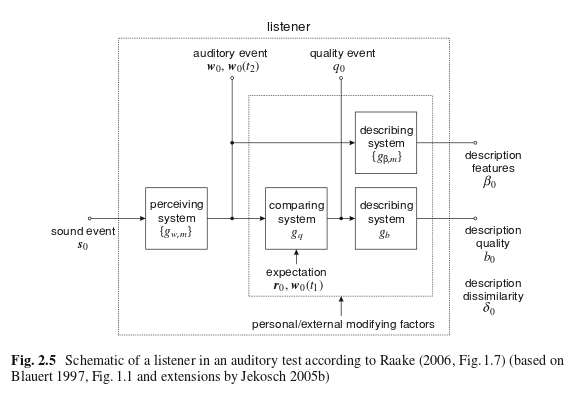
\includegraphics[width=1\textwidth]{figure/quality-event}
%	\caption{Quality formation and description process as extension to the perceptual event taken from \citet{waltermann_dimension-based_2013} after \citet{raake_short-_2006}.}
%	\label{img:chap02:quality-event} %Waeltermann, 2013
%\end{figure}
It is assumed that a perceptual event is evaluated by a \emph{comparing system} within the observer.
This system derives the \emph{quality features} of this event~\citep[\cf{}][p.\,17]{jekosch_voice_2005}.\footnote{\citet{jekosch_voice_2005} uses the term \emph{entity} with regard to the quality formation process.
As entity does not convey a temporal component, the term \emph{event} is in this work used instead; following the notion of \citet{blauert_spatial_1996}.}

\begin{definition}[Quality Feature]
``is a recognized and designated characteristic of an entity that is relevant to the entity's quality.''~\citep[][p.\,17]{jekosch_voice_2005}
\end{definition}

It is assumed that the evaluation of the difference between the \emph{perceived quality features} and the \emph{desired quality features} results in the experienced quality~\citep[p.\,23]{raake_quality_2014}.
With regard to telecommunication services and multimedia systems, the term \emph{perceived quality} has been extended to \acf{QoE}.
In \ac{QoE}, an observer is not regarded as an instrument of measurement, but as an \emph{actor} striving for a \emph{satisfying} perceived quality with regard to his expectations, requirements, and needs.
In difference to an observer, who only describes an event, an actor can proactively make decisions and react to his environment.  

\begin{definition}[\acl{QoE}]
``is the degree of delight or annoyance of a person whose experiencing involves an application, service, or system.
It results from the person’s evaluation of the fulfillment of his or her expectations and needs with respect to the utility and / or enjoyment in the light of the person’s context, personality and current state.''~\citep[][p.\,19]{raake_quality_2014}
\end{definition}

\citet{raake_quality_2014} extended the \emph{quality formation process} of \citet{jekosch_voice_2005}.
Here, both an anticipation process and an update process are added.
These processes incorporate current experiences into expectations and might result in an adjustment of the desired quality features.
Thus, the perceived quality of subsequent experiences might be affected.
In addition, the concept of \emph{assumed quality} is derived.
\begin{definition}[Assumed Quality]\label{def:assumedquality}
``corresponds to the quality and quality features that users, developers, manufacturers or service providers assume regarding a system, service or product that they intend to be using, or will be producing, without however grounding these assumptions on an explicit assessment of \textit{quality based on experiencing}.''~\citep[][p.\,17]{raake_quality_2014}.
\end{definition}
Here, the experience has not yet taken place, but the quality formation process is based on expectations and prior knowledge.
Based on \emph{assumed quality}, a user might decide to initiate an interaction or rather avoid it.

The actual experience and resulting perceived quality is affected by influence factors.
\begin{definition}[Influence Factor]
``Any characteristic of a user, system, service, application, or context whose actual state or setting may have influence on the \acl{QoE} for the user.''~\citep[][p.\,56]{reiter_factors_2014}
\end{definition}
Contextual factors, which include task, user behavior, and usage situation~\citep[][p.\,56]{reiter_factors_2014}, are important, as these are in general not invariant.
For example, high delay might not be noticed in a two\=/party telephone conversation if only one speaker is talking.
In such a case, the delay is not perceived as degradation and thus would not negatively affect the quality formation process.

The formation process of perceived quality is still under investigation because it is not yet fully understood. %TODO REF
In fact, assessment methods for perceived quality and the broader concept of \ac{QoE} are still under development.

\subsection{Assessment Methods}
For the assessment of perceived quality, experiments are conducted that allow an actor (\cf{} \autoref{related:perceivedQuality}) to use and thus experience a service or product.
Information about the quality of the experience can be derived by monitoring the actor, observing his behavior, or requesting him to describe his experience.

For a quantitative description scales with predefined labels are used often.
An actor describes his experience by selecting the label that closest characterizes his perceived quality.
The labels act as anchors, so multiple judgments of the same or different stimuli can be related to each other.
Examples of such scales are \acf{ACR} scales and \acf{CoCR} scales.
In the latter case, judgments between two labels can also be expressed.
%Most common is the 5\=/point \ac{ACR} ranging from \emph{Bad (1)} to \emph{Excellent (5)}. %\footnote{This scale is often denoted as \ac{MOS} scale. This however is not correct as the \ac{MOS} is rather the combination of multiple judgments by one or more actors into one score by calculating the arithmetic mean.}
%Note that the term stimulus is misleading as it suggests an observer rather than an actor, which in some cases might be correct but not in general.

Based on the judgments, a \acf{MOS} can be derived by averaging all judgments per stimulus \citep{itu-t_recommendation_p.800.2_mean_2013}.
The \ac{MOS} is assumed to reflect the judgment of an \emph{average actor} for this stimulus and the resulting experience.
Judgments of an experience can either be taken while experiencing (these being denoted as \emph{momentary judgments}) or after an experience.
Taking momentary judgments might affect the perceptual, quality formation, and descriptive processes, as the assessment task must be conducted in parallel. %TODO REF
However, momentary judgments allow the investigation of the impact of varying performance within a stimulus.
In fact, this allows the investigation of the noticeability of varying performance.
Assessing the perceived quality of an experience after this experience is denoted as \emph{retrospective judgment}~\citep[][]{weiss_temporal_2014}.
A retrospective judgment is based on recallable characteristics of an experience.
It has been observed that not all parts of an experience affect a retrospective judgment of this experience in a similar manner (\cf{} \autoref{chap:04}).
%For the investigation of the impact of small differences between stimuli often paired comparison methodologies are applied, which present multiple stimuli and request to judge them with regard to each other or select the \emph{better} one.

It must be noted that a judgment cannot be considered absolute in terms of being universal, as it is the result of the quality formation process and description process within the actor.
These processes are affected, for example, by differences in the so-called internal reference, which may lead to biases \citep[][]{zielinski_biases_2008, pitrey_aligning_2011}.
For example, narrowband speech stimuli are judged to be better if no wideband stimuli are presented \citep[][]{koster_comparison_2015}.

\subsection{Prediction of Perceived Quality}
Beyond understanding the underlying processes in detail, one major goal of research on \ac{QoE} is the algorithmic prediction of judgments.
This is especially important as the evaluation by humans is an expensive procedure and thus limits the number of evaluations.
In addition, continuous evaluation, as required for network monitoring, is not feasible in this manner.

An algorithmic predictor is called a \emph{model}.
A model maps the input, often a stimulus or an abstract reduced presentation of a stimulus, to the expected judgment.
The necessary information to create a model can be derived with subjective experiments, \ie, selecting \emph{representative} stimuli and letting participants judge the perceived quality.
A model can be applied for automatic evaluation, which is for example useful for the development of new coding algorithms.
Particularly in the case of telecommunication services, models have been developed for planning purposes, such as the \emph{E-Model} \citep{itu-t_recommendation_g.107_e-model_2015}.

%For the prediction of speech transmission and occurring degradations models have been developed 
%For speech transmission \ac{POLQA} \citep{itu-t_p.863:_2014} and \emph{E-Model} \citep{itu-t_g.107:_2015} are widely used examples.
%Where as the former predicts perceived quality based on the difference between input signal and output signal, the latter uses only a parametric, reduced representation.
%Depending on the purpose of a model, different input and outputs are desired.
%Input might also include beside technical performance-related characteristics, information about the influence factors.

In fact, a model is inherently limited by the underlying data which lead to the selection of the model's parts and parameters.
A model must be carefully applied to the implied restrictions resulting from the used data.
Using it outside its designed scope may result in invalid predictions.
